\chapter{Verification}

This purpose of this chapter is to outline the methods of verifying that the CoffeeBreak system implements the required features. The technologies used for verification, including frameworks, libraries, and services used, are all also outlined. Each successfully implemented feature requested has a section of this chapter dedicated, explaining how it has been verified, as well as potential flaws with the verification for that particular feature, or, should it be the case, why the particular feature has not been verified.

\section{Methodology and Technology}

For all JavaScript components, including the scripts in the browser-based clients, the testing framework Mocha is used, alongside the Chai assertion library, for both unit- and integration testing. GitHub Actions is used to automate the testing process through continuous integration (CI), in order to ensure everything pushed to the remote version control repository is tested.\footnote{True continuous integration tests are only done for a single component, the room repository, as a proof-of-concept. See the .github/workflows/integration.yml file in the repository repository for more information.} The one component implemented using Python, the media relay server, is merely tested using user acceptance test and thus does not use any particular technologies for testing, due to it being considered non-critical for the product itself, being merely an extra feature for the secondary project goal.

All unit and integration tests are available directly in the source code repositories, usually located in a folder called "test", "tests", or something similar, located in the root folder. This is with the single exception of the browser-based clients tests, which are located in the public/client\_test folder within the main controllers repository. Tests are usually split into multiple files, depending on what type of testing or which module is being tested.

The CI scripts are located under the .github/workflows folder from the root folder. These might not be visible by default in some operating systems, but can easily be located on the repository website.

\section{Requirement Verification}

This section lists all the requirements found during analysis, how they have been verified along with important code snippets. Each subsection is titled with the requirements ID and some context on what is being tested, loosely based on the original requirement description.

\subsection{R01 Pod-based Rooms}
\label{vR01}

Verified through running commands in the Kubernetes API, where it is possible to check running pods in the cluster. The socket-server, Heimdall, that handles room connections and messages sent to rooms is present as a deployment.

\subsection{R01.1 Room is Socket Server}
\label{vR01.1}

This is verified indirectly through the client integration tests, as they all emit and receive events to and from the room socket server. For instance, the following test in client integration tests ensure that the client has been assigned an ID, something which cannot occur without outside manipulation, unless the client has logged in to the room socket server.

\begin{lstlisting}[language=JavaScript]
it ('Logs in', async function () {
    await delayUntill (() => localUserId)
    expect(localUserId).to.exist
})
\end{lstlisting}

Note that the $delayUntill()$ function is merely a utility for awaiting until the given predicate holds true. It is used extensively in client integration tests, and in itself prohibits the tests from concluding before the condition holds true. With the Mocha testing framework, tests are automatically failed if not concluded within a given threshold, by default 2000ms.

\subsection{R01.2 Room Pods Automatically Created}
This requirement is fulfilled through the configuration of the Kubernetes deployment of the room socket server service. The deployment consists of a Replica Set, of which can create more replicas of itself depending on traffic and is verified through stress testing of the service. When the system was stress tested, the amount of pods increased to match the need.
\label{vR01.2}

\subsection{R02 Browser-based Room Client}
\label{vR02}

Verified in main controller integration tests for both endpoints GET /room and GET /room/:roomId, as well as a negative test of GET /room/:roomId, by asserting that the endpoints return an HTML document when expected. A snippet of code as an example of one of these test, this being for GET /room:

\begin{lstlisting}[language=JavaScript]
it ('GET /room', async function () {
    let response = await axios.get(url + '/room')
    expect(response.status).to.equal(200)
    expect(response.request.res.responseUrl).to.exist
    expect(response.data.startsWith('<!DOCTYPE html>')).to.be.true
})
\end{lstlisting}

While it is generally considered a good rule-of-thumb to only have a single assertion per test case, so that no two assertions are dependant on each other, this rule-of-thumb was not used in most tests primarily to avoid even more duplicate code that the tests already had.

\subsection{R02.1 Scalable Webserver}
Same verification method as R01.2
\label{vR02.1}

\subsection{R03 Connect to Rooms}
\label{vR03}

This is verified through the test case shown with R01.1 verification, see \ref{vR01.1}.

\subsection{R03.1 Room URL contains Room ID}
\label{vR03.1}

Verified in main controller integration tests of the GET /room/:roomId endpoint, where the test first requests a new room through GET /room, then requests the room using the redirect URL returned by GET /room. The returned URL is tested against a Regular Expression in order to verify that the URL contains a room ID.

\begin{lstlisting}[language=JavaScript]
it ('GET /room/:roomId', async function () {
    let response = await axios.get(url + '/room')
    let responseToRoom = await axios.get(response.request.res.responseUrl)

    let redirect = response.request.res.responseUrl
    let id = redirect.substring(redirect.lastIndexOf('/') + 1)

    const uuidRegex = /\b[0-9a-f]{8}\b-[0-9a-f]{4}-[0-9a-f]{4}-[0-9a-f]{4}-\b[0-9a-f]{12}\b/
    expect(uuidRegex.exec(id).length).to.equal(1)
    
    expect(responseToRoom.status).to.equal(200)
    expect(responseToRoom.data.startsWith('<!DOCTYPE html>')).to.be.true
})
\end{lstlisting}

\subsection{R03.2 Access Room Using ID}
\label{vR03.2}

Verified in the same test case as described for R03.1 above. See \ref{vR03.1}

\subsection{R03.3 Rooms Stored In Database}
\label{vR03.3}

As described in previous chapters, room storage is done through the room repository component. Each endpoint provided by the room repository is tested, including POSTing new rooms. Two tests, one for POSTing a new room, and one for getting a room with a particular ID verify this particular feature.

\begin{lstlisting}[language=JavaScript]
it ('POST /rooms', async function () {
    let post = await axios.post(url + '/rooms', {name: 'someName', socketUrl: 'http://someSocketUrl', signallingUrl: 'http://someSignallingUrl'})
    expect(post.status).to.equal(201)
})

it ('GET /rooms/:id', async function () {
    let post = await axios.post(url + '/rooms', {name: 'someName', socketUrl: 'http://someSocketUrl', signallingUrl: 'http://someSignallingUrl'})
    let room = await axios.get(url + '/rooms/' + post.data.id)

    éxpect(room.data.name).to.equal('someName')
    expect(room.data.socketUrl).to.equal('http://someSocketUrl')
    expect(room.data.signallingUrl).to.equal('http://someSignallingUrl')
    expect(room.status).to.equal(200)
})
\end{lstlisting}

Notice that the second test in this snippet both POSTs a new room as well as fetches it, as the database is cleaned up in between different tests. Both tests are still included to verified that the POST functionality works independently.


\subsection{R03.4 Requests Nickname on Room Join}
\label{vR03.4}

Verified by a small test from the browser-based clients integration tests. The testing client sets $window.prompt()$, the function used to prompt the user for a nickname, to always return "John Doe". After the user has logged in, it then verified that the user has logged in with the nickname "John Doe".

\begin{lstlisting}[language=JavaScript]
window.prompt = function(str) { return 'John Doe' } 
...
it ('Prompts nickname', async function () {
    expect(getLocalUser().nickname).to.equal('John Doe')
})
\end{lstlisting}

It is worth keeping in mind that this test occurs after the login test, meaning that the user is always logged in at this point. The testing framework runs all tests sequentially, regardless of any promises or any other sort of asynchronous programming. The two lines separated by three dots are not from the same file, they are merely displayed in the same snippet for brevity. The login occurs between the two parts of the code snippet.

\subsection{R04 Send Messages to Room}
\label{vR04}

This is verified through the clients integration testing with the room service. It sends a message with some dummy content to the room server, and awaits the message being added to the clients list of messages, then asserts that the content of the received message is what was originally sent.

\begin{lstlisting}[language=JavaScript]
it ('transmitChatMessage(author, content)', async function () {
    messages = []
    transmitChatMessage('someId', 'Some message content')
    await delayUntill(() => messages.length == 1)
    expect(messages[0].author).to.equal('someId')
    expect(messages[0].contents).to.equal('Some message content')
})

\end{lstlisting}

\subsection{R04.1 Messages Sent Through Room Service}
\label{vR04.1}

Already verified through the verification of requirement R04 just above, as it is through integration testing.

\subsection{R04.2 Users in Room Receives Message}
\label{vR04.2}

For the most part same as verification for R04.1. That other members of a room also receives the message is done through simple manual user acceptance testing.

\subsection{R05 Create Rooms}
\label{vR05}

While this is already tested by the main controller integration testing described with the verification for R02 and R03.1, their intent is mostly simply to test the main controller itself. Creating rooms is specifically tested through integration tests from the room manager, specifically the Odin room manager.

\begin{lstlisting}[language=JavaScript]
it ('POST /rooms', async function () {
    let response = await axios.post(url + '/rooms')
    expect(response.data.id).to.exist
    expect(response.status).to.equal(201)
})
\end{lstlisting}

The POST request returns the room and afterwards asserts that it exists through the room ID. The POST /rooms endpoint of the room repository is also tested in the repositories own testing.

\subsection{R05.1 Room Has Unique ID}
\label{vR05.1}

To verify this, 100 rooms are created in room repository tests, and all compared against every single other room to ensure that none of them share their ID.

\begin{lstlisting}[language=JavaScript]
it ('IDs are unique', async function () {
    posts = []
    for (let i = 0; i < 100; i++) {
        let post = await axios.post(url + '/rooms', {name: 'someName', socketUrl: 'http://someSocketUrl', signallingUrl: 'http://someSignallingUrl'})          
        posts.push(post)      
    }
    expect(posts.every(x => {
        let identicals = 0
        posts.forEach(y => {
            if (y.data.id == x.data.id) {
                identicals++
            }
        })
        return identicals == 1 // Each room will always come across itself.
    })).to.be.true
})
\end{lstlisting}

Notice that since UUIDs are used for room IDs, there is a infinitesimally small chance that two rooms actually do share their IDs, though in practice it can be safely assumed that this \textit{hopefully} will not occur within the lifetime of this universe.

\subsection{R06 Users Can Move}
\label{vR06}

This feature is verified through the integration testing of the browser-based client. Similarity to verifying R04, this is done by sending the movement request and awaiting the response from the room service.

\begin{lstlisting}[language=JavaScript]
it ('moveLocalUser (x, y)', async function () {
    moveLocalUser(300, 300)
    await delayUntill(() => getLocalUser().x == 300)
    expect(getLocalUser().x).to.equal(300)
    expect(getLocalUser().y).to.equal(300)
})
\end{lstlisting}

\subsection{R06.1 Users Move By Clicking Canvas}
\label{vR06.1}

This is merely verified through manual user acceptance testing, due to the feature being dependant with directly handling an event raised by the canvas itself. This could potentially be made more testable by splitting the handling of the event and the computation of movement in two different functions, but even so, the verification of clicking would only truly be verified by an actual click.

\subsection{R06.2 User Movement Sent to Room Members}
\label{vR06.2}

To some extend already verified by the verification of R06, though it is further verify by simple manual user acceptance testing.

\subsection{R06.3 Room Members Movement Sent to User}
\label{vR06.3}

Same as R06.2.

\subsection{R06.4 Movement Updates Nearby Users}
\label{vR06.4}

This has proven difficult to verify using automated testing methods alongside the rest of the tests, as it effectively requires two clients due to the implementation, something which could easily interfere with other tests. However, it can easily be verified by manually verifying by logging two browsers in to the same room, moving each avatar close to each other, and executing $console.log(nearby)$ in the browser console, and verifying that there is a single element within the array. This is shown in figure \ref{fig:verifiednearby}.

\begin{figure}[H]
    \centering
    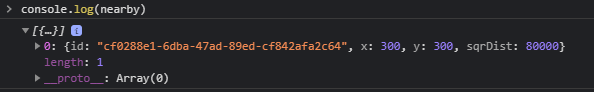
\includegraphics[width=\textwidth]{Pictures/ValidateNearby.png}
    \caption{Image showing the execution of $console.log(nearby)$ after two browsers joined the same room and moved near to each other. Shows how the printed object contains a single "nearby" user. The actual numbers should be disregarded.}
    \label{fig:verifiednearby}
\end{figure}

There was an actual test case implemented for this particular feature, but it was deeply flawed and would always pass no matter the state of the system, it has since been removed but can be found in previous versions of the system.

\subsection{R07 Video and Voice Connection}
\label{vR07}

This particular feature is not automatically tested due to the complexity of setting up such a test, as well as the many unknowns involved. Through manual user acceptance testing, the feature is deemed \textit{verified enough}. It can be verified that a connection is established by examining the chrome://webrtc-internals/ page included with Google Chrome. This page includes a large amount of information about current WebRTC connections.

\subsection{R07.1 WebRTC Connection}
\label{vR07.1}

Same as R07.

\subsection{R07.1.1 Signalling Server}
\label{vR07.1.1}

Signalling is verified in the client integration tests, by sending a message to itself through the signalling server, and waiting for a response, effectively pinging the signalling server. 

\begin{lstlisting}[language=JavaScript]
it ('sendMessage(...)', async function () {
    await delay(1000)
    let response;
    signalling.on('message', message => {
        response = message;
    })
    sendMessage({ type: 'type', contents: 'contents' }, localUserId)
    await delayUntill(() => response)
    expect(response.message.type).to.equal('type')
    expect(response.message.contents).to.equal('contents')
})
\end{lstlisting}

\section{Conclusion}

For almost all components in the system, the Mocha testing framework is used alongside the Chai assertion library. This holds true even for the browser-based client. For continuous integration, GitHub Actions is used to automate the testing process. The one component not written in JavaScript has not been tested, as it is not considered critical for the project itself, instead being an extra feature. The large majority of requirements has been verified through unit- or integration tests, with a few exceptions due to prohibitive complexity, or some other reason. These are merely verified through manual user acceptance test or an arbitrary manual testing method.